Personal Learning Networks are the collections of people and information
resources (and relationships with them) that people cultivate in order
to form their own public or private learning networks --- living,
growing, responsive sources of information, support, and inspiration
that support self-learners.

\begin{quote}
\textbf{Howard Rheingold}: ``When I started using social media in the
classroom, I looked for and began to learn from more experienced
educators. First, I read and then tried to comment usefully on their
blog posts and tweets. When I began to understand who knew what in the
world of social media in education, I narrowed my focus to the most
knowledgeable and adventurous among them. I paid attention to the people
the savviest social media educators paid attention to. I added and
subtracted voices from my attention network, listened and followed, then
commented and opened conversations. When I found something I thought
would interest the friends and strangers I was learning from, I passed
along my own learning through my blogs and Twitter stream. I asked
questions, asked for help, and eventually started providing answers and
assistance to those who seemed to know less than I. The teachers I had
been learning from had a name for what I was doing --- ``growing a
personal learning network.'' So I started looking for and learning from
people who talked about HOW to grow a ``PLN'' as the enthusiasts called
them.''
\end{quote}

\subsubsection{Strong and weak ties}

Your PLN will have people and sites that you check on often -- your main
sources of information and learning -- your `strong ties'. Your `weak
ties' are those people and sites that you don't allow a lot of bandwidth
or time. But they may become strong later, as your network grows or your
interests expand. This is a two-way street -- it is very important that
you are sharing what you learn and discover with those in your network
and not just taking, if you want to see your network expand.

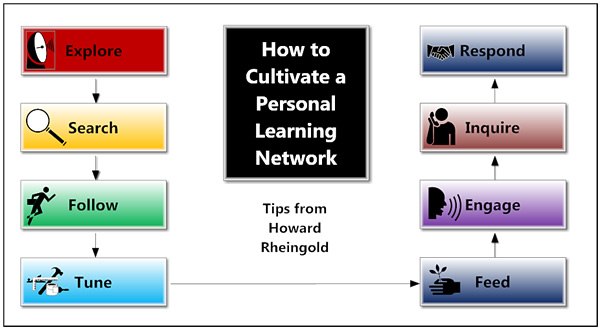
\includegraphics{http://peeragogy.org/wp-content/uploads/2013/09/cultivate.jpeg}

\subsubsection{Peer learning networks}

As you convene your peer learning group, in one form or another you will
develop and share ``peeragogical profiles'' --- advertising what you
want to learn, what you'd be interested in helping teach others. If you
present yourself and your projects in a thoughtful and engaging way,
this will help you to build effective connections. Networks of these
connections can span across different subjects, across a city, or across
national boundaries.~ Peeragogy helps to make sense of the idea of
``learning networks'' that has been around since at least the 1970s.~
Much as theories of pedagogy would be relevant for anyone carefully
planning an individual learning programme, peeragogy is relevant for
self-organized learning communities operating at larger scales.
